% a=10,b=8,c=6. Wrong cyclic weights give J=(bA+cB+aC)/24=(3/2,10/3).
\begin{center}
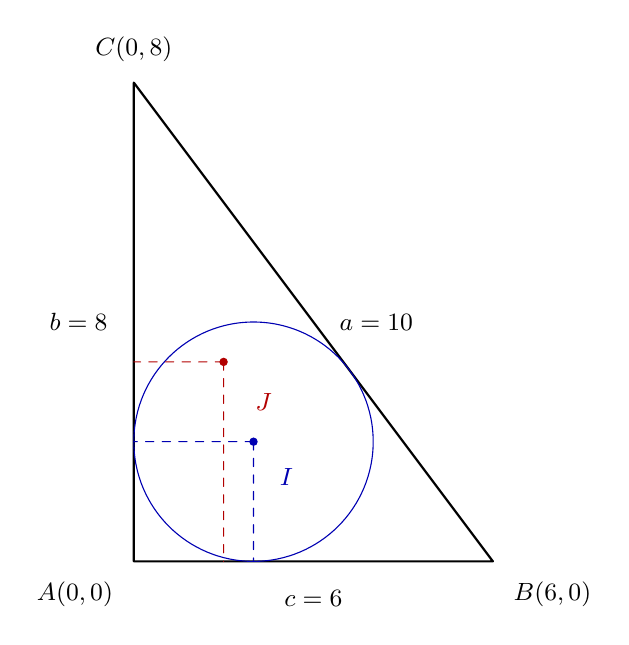
\begin{tikzpicture}[scale=.76,font=\small,line cap=round,line join=round]
\coordinate (A) at (0,0);\coordinate (B) at (6,0);\coordinate (C) at (0,8);
\coordinate (I) at (2,2);\coordinate (J) at (1.5,10/3);
\draw[thick] (A)--(B)--(C)--cycle;
\draw[blue!70!black] (I) circle[radius=2];
\draw[blue!70!black,dashed] (I)--(2,0) (I)--(0,2);
\draw[red!70!black,dashed] (J)--(1.5,0) (J)--(0,10/3);
\fill[blue!70!black] (I) circle[radius=2pt];\node[below right=6pt,blue!70!black] at (I) {$I$};
\fill[red!70!black] (J) circle[radius=2pt];\node[below right=8pt,red!70!black] at (J) {$J$};
\node[below left=4pt] at (A) {$A(0,0)$};\node[below right=4pt] at (B) {$B(6,0)$};\node[above=4pt] at (C) {$C(0,8)$};
\path (B)--node[midway,right=6pt] {$a=10$} (C);
\path (C)--node[midway,left=6pt] {$b=8$} (A);
\path (A)--node[midway,below=7pt] {$c=6$} (B);
\end{tikzpicture}
\par\smallskip{\small 正确内心 $I(2,2)$；错配系数得到 $J(3/2,10/3)$，它到两坐标轴的距离都不相等。}
\end{center}
